%!TEX root = base.tex

\chapter{Previous Work}

Modelling of Wi-Fi performance has been an active field of research and this
chapter provides an introduction to the modeling approach described by Bianchi
\cite{bianchi} and subsequent efforts to improve it made by others. In
particular, the studied model presented by Ekici \& Felemban \cite{felemban}
will be discussed.

As mentioned previously, the IEEE 802.11 family specifies the PHY and MAC
layers of WLANs. Analysing the performance impact of these protocols, and 
their numerous parameters, is key to improving network performance. There are
two possible paradigms available: measuring/sampling or constructing an
analytic model of the system/property. Measuring can be done directly on both
physical hardware and software simulations whereas analytical models provide
performance figures as solutions of equations.

The complete behavior of the IEEE 802.11 standards have yet to be captured by
any single analytic model, and researchers instead take the standard
scientific approach of solving a constrained variant of the problem, which in
turn requires rigorous validation of the solution. A model may perform well in
certain conditions and pathologically in others. These behavioural
pecularities arrise from simplification of system behaviour and properties. In
a given model, simplifications can also be inherent in the original
construction mechanism—the way the model itself was constructed—which forces
the model itself to undergo a sort of ironic self-analysis and validation.
Model authors typically present a validation effort to prove their model's
credibility, which further requires scrutiny of the validation itself,
possibly in absurdum...

In short, model authors try to describe a complex system by modelling key
components in a constrained setting, and validate their model using other
models which have been more thoroughly reviewed. 

Given this context, we first present the original Markov-Chain model from
\cite{bianchi} and describe how it models IEEE 802.11 properties using the
DCF, some significant and intentional simplifications made and a narrow
selection of subsequent contributions made by others $refs$. % TODO: ADD REFS

Finally, the evaluated model \cite{felemban} is described as well as the
differences to both the original model \cite{bianchi} and some intrinsic model
properties useful in forthcoming chapters.

\section{The Bianchi Model}

In \cite{bianchi}, Bianchi presented a novel approach to modeling IEEE 802.11
performance by creating a Markov chain model of the \emph{Distributed
Coordination Function} (DCF). Bianchi defines three important properties:
transmission probability, normalised throughput and channel access delay. This
section provides a summary of the original model and definitions useful in
later chapters.

Before going into detail about the Bianchi model, we start from the beginning.

The underlying assumption of a MAC-layer-based model of IEEE 802.11 is that,
in a setting with more than 2 STAs, the MAC protocol should be the system
bottleneck. By extension, it is reasonable to model the performance of the
network based on the DCF. 

In \cite{bianchi}, Bianchi starts by limiting the proposed model analysis to
fully-connected, single-hop networks in ``saturation''. The saturation
condition requires that all STAs, at any point in time, always want to
transmit. This allows Bianchi to omit send queue distributions and simplify
collision probabilities, which will become important. Additionally, Bianchi
assumes that there is a fixed number of $N$ equivalent, contending STAs.

The back-off counter for a given STA at time $t$ is represented by the
stochastic process $b(t)$. Since the back-off counter at any given time $t$ is
dependent on the transmission history it follows that $b(t)$ is non-Markovian.
To solve this problem Bianchi assumes that each transmission attempt collides
with a constant and independent probability $p$.

In addition to the back-off counter process, $b(t)$, Bianchi also introduces a
stochastic process $s(t)$ representing the current back-off stage for a given
STA at time $t$. Recall from Equation \ref{eq:mlog} that $m$ is the number of
back-off stages, from which the states of $s(t)$ can be obtained as $(0,
\dots, m)$.

After breaking the historical dependency of the back-off process, Bianchi can
model the time-discrete bidimensional process $\{s(t), b(t)\}$ as the Markov
chain seen in Figure \ref{fig:tnmc}. As seen in the figure, the model ignores
several important behaviors of the DCF, in particular retransmission limit and
backoff counter freezing due to channel state.

\begin{enumerate}

	\item \textbf{Retransmission Limit} - the model does not drop the packet
after failing \texttt{ShortRetryLimit} retransmissions, instead it continues
until the packet has been successfuly acknowledged.

	\item \textbf{Back-off Counter Freezing} - in each back-off state, the
probability of decrementing the back-off counter—equivalent to sensing the
channel idle—is always 1.

\end{enumerate}

Bianchi assumes that the conditional collision probability $p$ is constant and
independent of the back-off stage. This implies that $p$, the probability of
an STA encountering collision during transmission, is equivalent to the
probability that any of the other $N-1$ STAs also attempted to transmit, with
transmission probability $\tau$

\begin{equation} \label{eq:pbi}
	p = 1 - (1 - \tau)^{N-1}
\end{equation}

By modelling the back-off counter itself, combined with the saturation
condition and omission of retransmission limit, Bianchi solves the
transmission probability $\tau$ by essentially finding the steady state
probability of the back-off counter being zero, and obtains

\begin{equation} \label{eq:xbi}
	\tau = \frac{2(1-2p)}{(1-2p)(\mathit{CW_{min}}+1)+p\mathit{CW_{min}}(1-(2p)^m)}
\end{equation}

However, since $\tau$ is derived from the back-off counter, and the back-off
counter depends on the conditional collision probability $p$, it follows that
$\tau$ and $p$ are recursively defined. Bianchi constructs a nonlinear system
with equations for $\tau$ and $p$ and solves it numerically.

With probabilities for $\tau$ and $p$, Bianchi continues to his core
contribution—the normalised throughput. Denoted $S$, it is defined as ``the
fraction of time the channel is used to transmit payload bits''. 

\begin{equation} \label{eq:ssbi}
	S = \frac{E[\mathit{payload~information~transmitted~in~a~slot~time}]}{E[\mathit{length~of~slot~time}]}
\end{equation}

With $E[P]$ denoting mean payload size, probabilities for transmission
$P_{tr}$ and transmission success $P_S$, the numerator in \ref{eq:ssbi}
becomes $P_S P_{tr} E[P]$. In a similar fashion, the denominator in
\ref{eq:ssbi} can be expressed as the sum of empty time slots, busy time slots
and times slots with collisions. Let $\sigma$ be the duration of an empty
slot, $T_{S}$ the average time the channel is sensed busy in case of
successful transmission, and $T_{C}$ the average time the channel is sensed
busy in case of collision for the non-colliding STAs. Now, Bianchi presents an
equation for the normalized througput $S$

\begin{equation} \label{eq:sbi}
	S = \frac{P_S P_{tr} E[P]}{(1-P_{tr})\sigma + P_{tr} P_S T_S + P_{tr} (1-P_S) T_C}
\end{equation}

Note that $S$ is expressed independent from the ``access modes'' found in
Figure \ref{fig:timings}, which details the communication flow of a single,
successful packet transmission and acknowledgement. Let $H = T_{\mathit{PHY}}
+ T_{\mathit{MAC}}$ and assume propagation delay $\delta$. The differences
between the ``access modes'' can thus captured by the variables $T_{S}$ and
$T_{C}$

\begin{align}  \label{eq:tbi}
	\mathit{basic} & \left\{
		\begin{aligned}
	        T^{bas}_{S} & = H + E[P] + \mathit{SIFS} + \delta + \mathit{ACK} + \mathit{DIFS} + \delta  \\
	        T^{bas}_{C} & = H + E[P] + \mathit{DIFS} + \delta
	    \end{aligned}
	\right. \\
	\mathit{RTS/CTS} & \left\{
	    \begin{aligned}
	        T^{rts}_{S} = & ~ \mathit{RTS} + \mathit{SIFS} + \delta + \mathit{CTS} + \mathit{SIFS} + \delta \\ & + H + E[P] + \mathit{SIFS} + \delta + \mathit{ACK} + \mathit{DIFS} + \delta  \\
	        T^{rts}_{C} = & ~ \mathit{RTS} + \mathit{DIFS} + \delta
	    \end{aligned}
	\right.
\end{align}


From these equations Bianchi concludes that for any network of size $N$ there
exists a troughput-optimal transmission probability $\tau$, achievable by
tuning the congestion window sizes and $\mathit{CW_{min}}$ and $\mathit{CW_{max}}$.

To make the model tractable Bianchi simplifies many behaviours, of which two
have received considerable efforts to implement. Some notable publications 
are Wu \cite{1019305} and Chatzimisios \cite{1258379}, who proposed improved
models that included the retransmission limit, followed by Zhang
\cite{article} and Xiao \cite{1512111}, who proposed models that include
back-off counter freezing.

\begin{figure}
\center
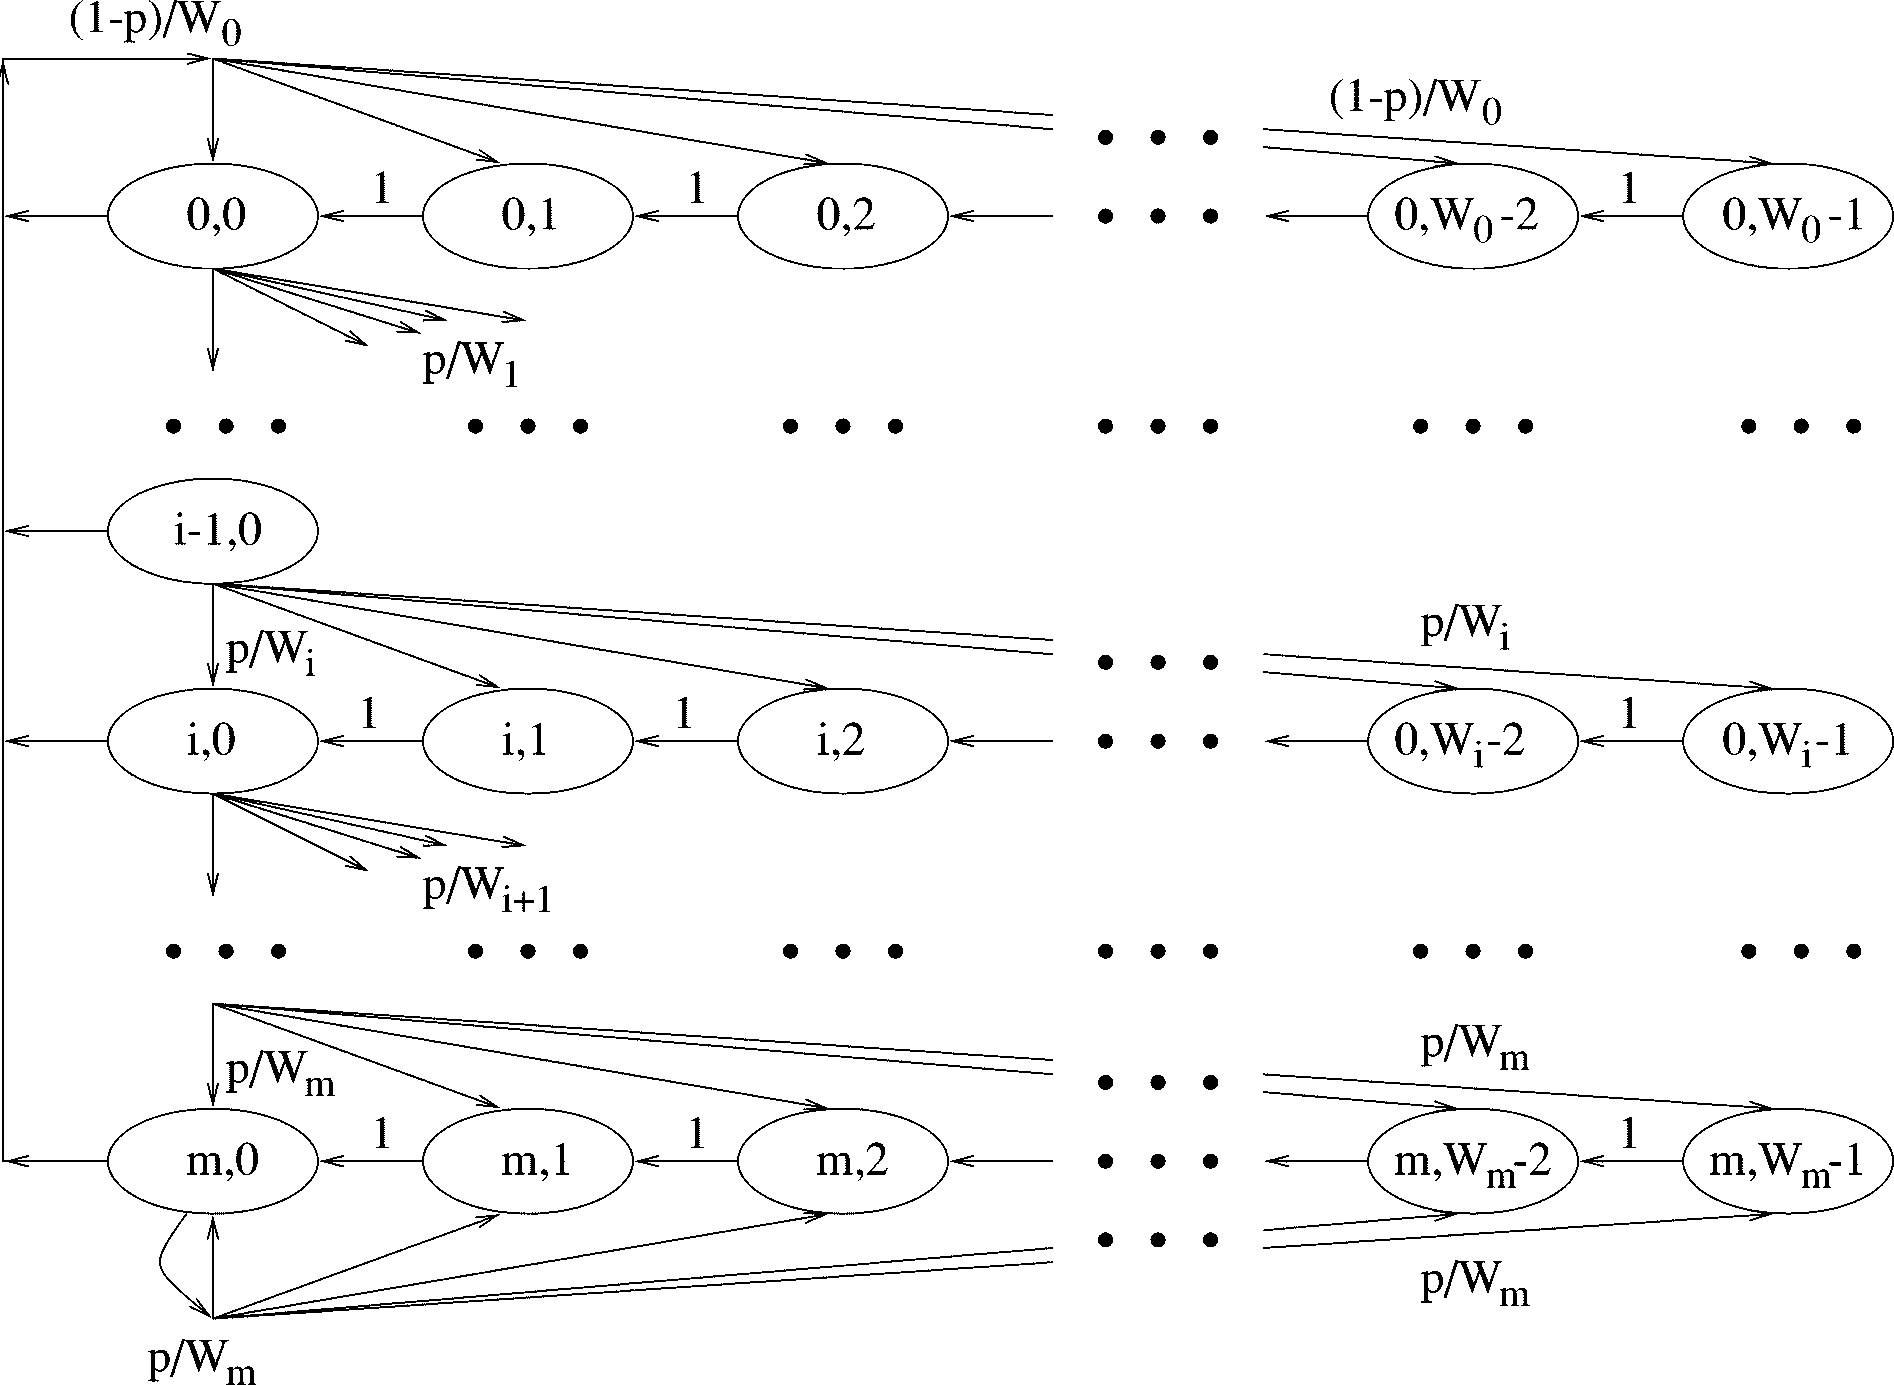
\includegraphics[width=0.9\textwidth]{images/bianchi-model.png}
\caption{Bianchi's \emph{Tagged-Node Markov Chain} model of the IEEE 802.11 DCF where $p$ is the collision probability, $W_i$ the contention window size at attempt $i$ ($0 \leq i \leq m$) and $m$ from Equation \ref{eq:mlog}.}
\label{fig:btnmc}
\end{figure}

\section{The Felemban-Ekici Model}

A decade later, in 2011 specifically, Felemban \& Ekici published an extended
version of Bianchi's model, where they significantly improved the model's
accuracy by introducing a more accurate behaviour of the entry into backoff
and the backoff countdown procedures \cite{felemban}.

An overview of the TNMC model from \cite{felemban} is presented in Figure
\ref{fig:tnmc}. Some differences compared to Bianchi's TNMC are inclusion of
retransmission limit (in state $\{0,L\}$, collision results in packet drop)
and counter freezing $P_f$ (probability of state a $\{i,j\}$ transitioning to itself).

The inclusion of retransmission limits results in a different expression of
$\tau$ compared to Equation \ref{eq:xbi}. Recall from Equation \ref{eq:cwj}
that $W_j$ is the size of the contention window at back-off stage $j$ and that
$L$ is the short retry limit from \cite{654749}. Felemban \& Ekici solves
$\tau$ similarly to \cite{bianchi} by finding the probability of the back-off
counter reaching 0 in all back-off stages, expressed as

\begin{equation} \label{eq:xfe}
	\tau = \frac{1-P^{L+1}}{
		(\Sigma^L_{j=0}
			[1 + \frac{1}{1-P_f}
				\Sigma^{W_j-1}_{k=1} \frac{W_j-k}{W_j}
			]
		)(1-P)}
\end{equation}

where $P$ is the conditional collision probability (equivalent to $p$) from
Equation \ref{eq:pbi}.

\begin{align}  \label{eq:tfe}
	\mathit{basic} & \left\{
	        T^{bas}_{C} = T^{bas}_{S} = \mathit{DIFS} + T_h + T_p + \mathit{SIFS} + \mathit{ACK}
	\right. \\
	\mathit{RTS/CTS} & \left\{
	    \begin{aligned}
	        T^{rts}_{S} = & ~ \mathit{DIFS} + T_\mathit{RTS} + \mathit{SIFS} + T_\mathit{CTS} \\ & + \mathit{SIFS} + T_h + T_p + \mathit{SIFS} + \mathit{ACK}  \\
	        T^{rts}_{C} = & ~ \mathit{DIFS} + T_\mathit{RTS} + \mathit{SIFS} + T_\mathit{CTS}
	    \end{aligned}
	\right.
\end{align}

As shown in Figure \ref{fig:dcfgraph}, the DCF back-off process algorithm
specifies that a node only decrements the back-off counter if the channel was
sensed idle. In \cite{felemban}, the authors obtained an accurate countdown
probability ($P_d$) by introducing an additional markov chain to model the
channel-sensing process and estimating the probability of \emph{not} counting
down, i.e. probability of counter freeze ($P_f$). This chain is called
Channel-Sense Markov Chain (CSMC). The counter freeze probability, $P_f$, is
computed by finding the steady state probabilities of the CSMC by fixed point
iteration.

The addition of CSMC and $P_f$ increased the model's accuracy significantly
compared to other models in various test conditions. In particular, the
introduction of $P_f$ increased accuracy of the model when extended to
\emph{unsaturated} networks.

While the model proposed by Ekici-Felemban models the DCF more closely and
accurately, several assumptions and omissions, in addition to constraints
inherited from the markov chain approximation, makes the model a very
interesting candidate for real-world testing. 

\begin{figure}
\center
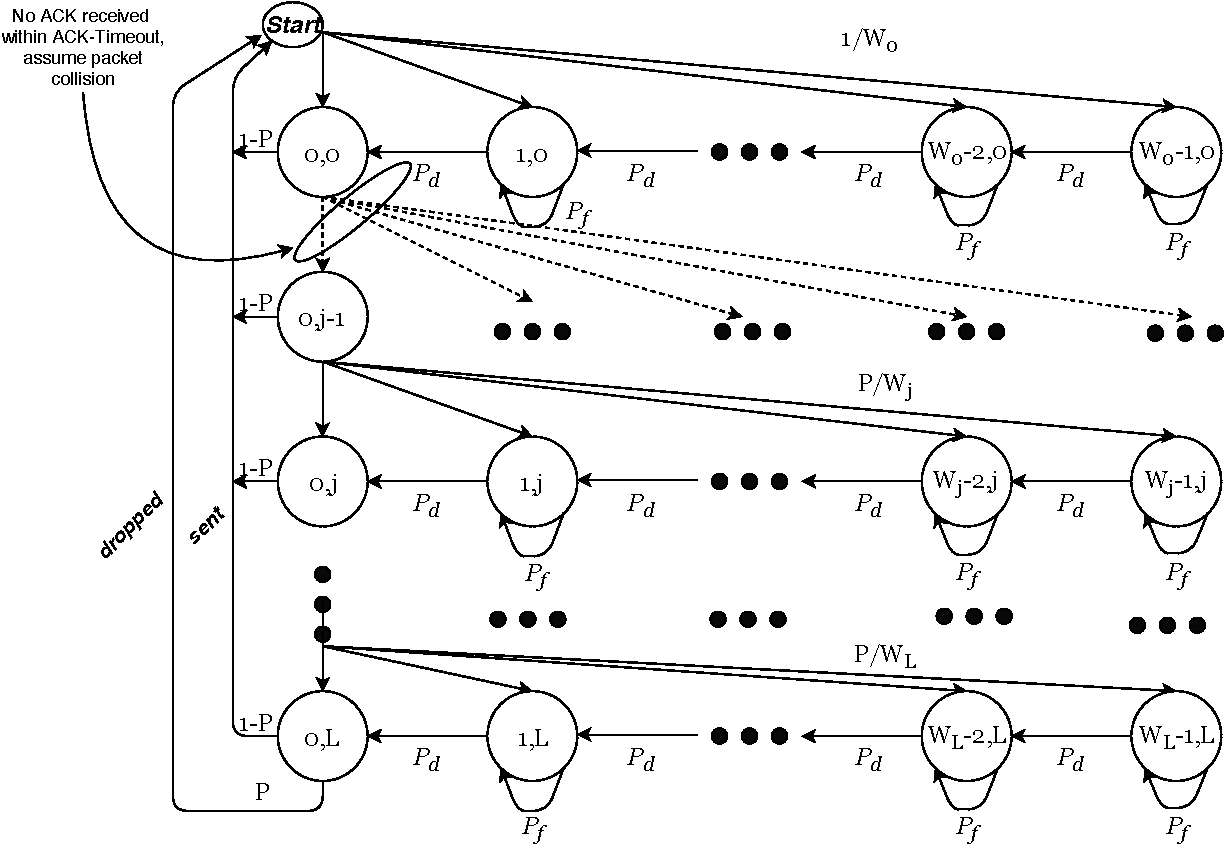
\includegraphics[width=1\textwidth]{images/tnmc-dcf.pdf}
\caption{Ekici-Felemban's Tagged-Node Markov Chain (TNMC) model of the IEEE 802.11 DCF. $P$ is packet collision probability, $P_d$ is probability to decrease backoff counter, $P_f = 1 - P_d$, $W_j$ is contention window size at attempt $j$ and $L$ is the Short Retry Limit}
\label{fig:tnmc}
\end{figure}

\subsection{The Unsaturated Model}

Recall that the original Bianchi model assumed that the network was in
\emph{saturation} conditions, i.e. all STAs always have something in their
send buffer. After presenting the improved model in \cite{felemban}, 
extended to work in \emph{unsaturated} networks.